\chapter{Preliminaria}
Aby zrozumieć jak działa dostarczony serwer, należy wpierw zrozumieć architekturę rozszerzenia w systemie edytora Visual Studio Code, a także na czym polega omawiany protokół. W tym rozdziale poruszone zostaną:

\begin{itemize}
    \item Visual Studio a Visual Studio Code.
    \item Struktura wtyczki rozszerzającej działanie edytora.
    \item Opis protokołu LSP.
    \item Parser Luaparse.
\end{itemize}

\section{Visual Studio (Code)}
Wiele osób nie rozróżnia od siebie dwóch produktów Microsoftu. Visual Studio to zintegrowane środowisko programistyczne, nastawione głównie na pisanie programów w języku C\#. Visual Studio Code jest natomiast edytorem kodu o otwartym kodzie opartym na silniku renderującym Electron od portalu Github, co sprawia, że jest on dosyć podobny do edytora Atom (również pod względem metodologii wtyczek). Dużą zaletą VS Code jest wbudowane wsparcie dla języków JavaScript i TypeScript, oraz środowiska Node.js, co przełożyło się na znaczny wzrost liczby użytkowników w ciągu 2 lat od powstania edytora (ponad 2,6 miliona aktywnych użytkowników \cite{connect})

\section{Struktura rozszerzenia Visual Studio Code}
Sercem każdego rozszerzenia jest plik \texttt{package.json}, który przechowuje informacje na temat autora pakietu, warunki jego uruchomienia, a także wszystkie jego zależności:

\begin{lstlisting}[language=JavaScript, basicstyle=\fontsize{9}{10}\ttfamily]
    {
        "name": "lua-lang",
        "description": "Lua language support",
        "author": "Wiktor Adamski",
        "license": "MIT",
        "version": "0.0.1",
        "engines": {
            "vscode": "^1.16.0"
        },
        "categories": [
            "Languages"
        ],
        "activationEvents": [
            "onLanguage:lua"
        ],
        "main": "./out/src/extension",
        "contributes": {
            "languages": [
                {
                    "id": "lua",
                    "aliases": [
                        "Lua",
                        "lua"
                    ],
                    "extensions": [
                        ".lua",
                        ".p8",
                        ".rockspec"
                    ],
                    "configuration": "./language-configuration.json"
                }
            ],
        },
        "dependencies": {
            "vscode": "^1.1.5",
            "vscode-languageclient": "^3.4.2"
        }
    }
\end{lstlisting}

O ile serwer LSP może być napisany w dowolnym języku, część bezpośrednio łącząca się z edytorem (aktualna wtyczka) musi być w języku JavaScript dla środowiska uruchomieniowego Node.js. 

Duża część kodu który jest wspólny dla wszystkich rozszerzeń jest możliwa do automatycznego stworzenia przez generator kodu Yeoman. Polecenie \texttt{yo code} przeprowadzi nas przez kreator wtyczek i utworzy dodatkowe pliki konfiguracyjne, które pozwolą korzystać z edytora VS Code jako środowiska developerskiego.

\section{Protokół Language Server Protocol}
Protokół LSP \cite{docs} jest specjalizacją protokołu JSON-RPC, który przesyła dane między stronami komunikacji za pomocą obiektów JSON. Klient (rozszerzenie edytora kodu) wysyła zapytania do serwera (program wspomagający) odpowiadające różnym akcjom podejmowanym przez programistę, np. zapytanie się o miejsce deklaracji danej zmiennej.

\begin{figure}[H]
    \centering
    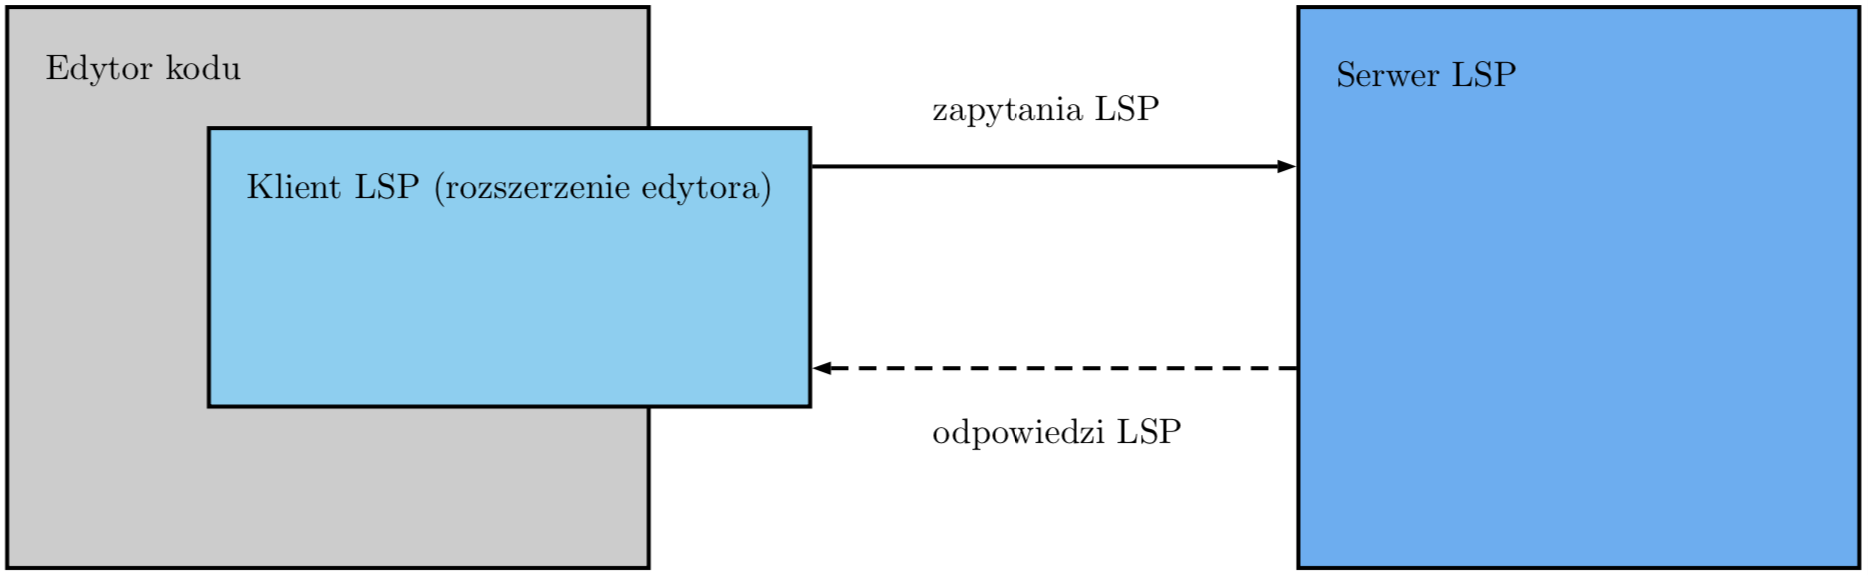
\includegraphics[scale=0.4]{Chapters/graf_komunikacji}
\end{figure}

Pierwszą wiadomością w trakcie połączenia jest wymiana możliwości zarówno klienta (np. czy edytor wspiera przemianowanie zmiennej), jak i serwera (np. wskazanie definicji danego symbolu lub automatyczne uzupełnianie pisanego tekstu). Twórcy protokołu udostępnili bibliotekę bibliotekę ułatwiającą korzystanie z niego w języku TypeScript. Poniżej przedstawiam przykładowy komunikat klienta informujący o otwarciu pliku w edytorze:

\begin{lstlisting}[language=JavaScript]
    {
        "jsonrpc": "2.0",
        "id": 1,
        "method": "textDocument/didOpen",
        "params": {
            "uri": "/Users/wiktor/Desktop/test.lua",
            "languageId": "lua",
            "version": 1,
            "text": "w = 'hello world'\nprint(n)"
        }
    }
\end{lstlisting}

W odpowiedzi serwer wyśle następujący komunikat z informacją o braku błędów w pliku:

\begin{lstlisting}[language=JavaScript]
    {
        "jsonrpc": "2.0",
        "id": 2,
        "method": "textDocument/publishDiagnostics",
        "params": {
            "uri": "/Users/wiktor/Desktop/test.lua",
            "diagnostics": []
        }
    }
\end{lstlisting}

Kontynuując, klient może wysłać zapytanie na temat definicji danego symbolu:

\begin{lstlisting}[language=JavaScript]
    {
        "jsonrpc": "2.0",
        "id": 3,
        "method": "textDocument/definition",
        "params": {
            "uri": "/Users/wiktor/Desktop/test.lua",
            "position": {
                "line": 1,
                "character": 7
            }
        }
    }
\end{lstlisting}

Przy odpowiadaniu serwer musi stwierdzić co znajduje się na podanej w zapytaniu pozycji (w tym przykładzie zmienna \texttt{n}) i zwrócić miejsce w pliku gdzie została zadeklarowana:

\begin{lstlisting}[language=JavaScript]
    {
        "jsonrpc": "2.0",
        "id": 3,
        "result": {
            "uri": "/Users/wiktor/Desktop/test.lua",
            "range": {
                "start": {
                    "line": 0,
                    "character": 0
                },
                "end": {
                    "line": 0,
                    "character": 0
                }
            }
        }
    }
\end{lstlisting}

W powyższej odpowiedzi został zwrócony fragment długości 0, co daje znać edytorowi by zaznaczył całe słowo zawierające daną pozycję.

\section{Biblioteka Luaparse i drzewa rozbioru}
Aby dostarczać jakiekolwiek sensowne informacje na temat kodu, potrzebne jest jego sparsowanie. Zajmuje się tym biblioteka Luaparse \cite{luaparse}, która produkuje abstrakcyjne drzewa rozbioru programów napisanych w języku Lua. Drzewa reprezentowane za pomocą obiektów JavaScript są inspirowane na specyfikacji Mozilla Parser API. Przykładowo wyrażenie:

\begin{lstlisting}[language={[5.3]Lua}]
foo = "bar"
\end{lstlisting}
zostanie przełożone na następujące drzewo:

\begin{figure}[H]
    \centering
    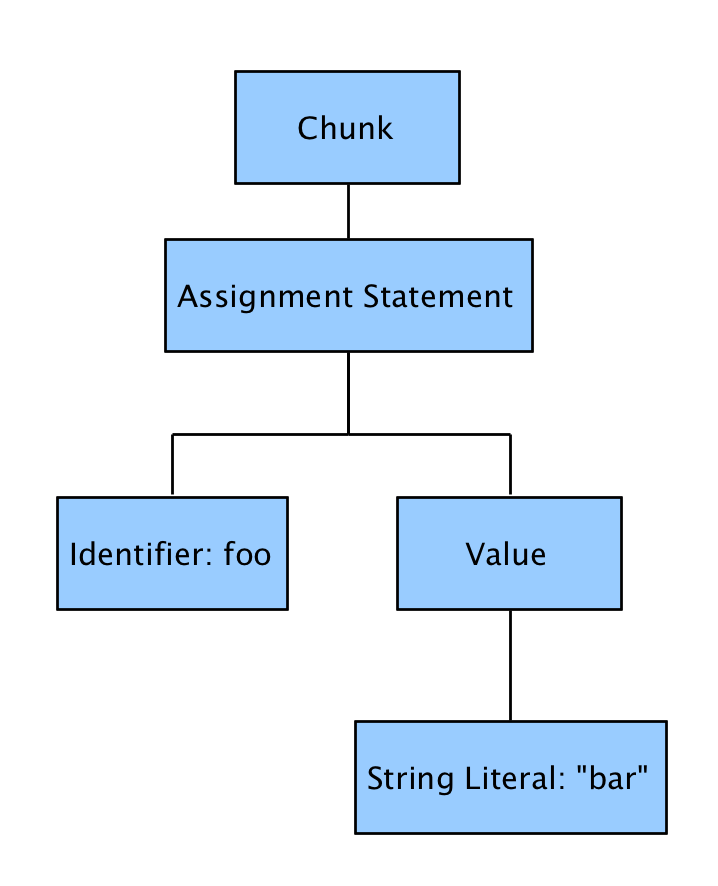
\includegraphics[scale=0.6]{Chapters/ast}
    \end{figure}

Powstałe drzewo jest później wykorzystywane do wyliczania odpowiedzi na zapytania klienta LSP, np. posłuży do odnalezienia miejsca definicji zmiennej o którą pyta się użytkownik rozszerzenia.
